\documentclass[12pt,a4paper]{article}
\usepackage[utf8]{inputenc}
\usepackage[T1]{fontenc}
\usepackage{geometry}
\usepackage{amsmath}
\usepackage{booktabs}
\usepackage{array}
\usepackage[table]{xcolor}
\usepackage{pgfplots}
\usepackage{pgfplotstable}
\usepackage{tikz}
\usepackage{graphicx}
\usepackage{float}
\usepackage{caption}
\usepackage{parskip}
\usepackage{fancyhdr}
\usepackage{titlesec}
\usepackage{hyperref}
\usepackage{listings}
\usepackage{xcolor}

\lstset{
  language=Python,
  basicstyle=\small\ttfamily,
  keywordstyle=\color{blue},
  commentstyle=\color{gray},
  stringstyle=\color{red},
  breaklines=true,
  captionpos=b,
  tabsize=2,
  showstringspaces=false,
  frame=single,
  rulecolor=\color{lightgray}
}

\pgfplotsset{compat=1.18}

\geometry{
  top=2.5cm, bottom=2.5cm,
  left=2.5cm, right=2.5cm
}

% Colors
\definecolor{javblue}{RGB}{0,0,0}
\definecolor{lightblue}{RGB}{208,228,247}
\definecolor{rowgray}{RGB}{245,245,245}
\definecolor{lightgray}{RGB}{200,200,200}

% Section formatting
\titleformat{\section}{\large\bfseries\color{javblue}}{}{0em}{}[\color{javblue}\titlerule]
\titleformat{\subsection}{\normalsize\bfseries\color{javblue}}{}{0em}{}
\titlespacing{\section}{0pt}{14pt}{6pt}
\titlespacing{\subsection}{0pt}{10pt}{4pt}

% Header/footer
\pagestyle{fancy}
\fancyhf{}
\fancyhead[L]{\small\color{javblue}Administracion de Bases de Datos}
\fancyhead[R]{\small\color{javblue}Semana 2 - Carga de Datos}
\fancyfoot[C]{\small\thepage}
\renewcommand{\headrulewidth}{0.4pt}

\hypersetup{colorlinks=true, linkcolor=javblue, urlcolor=javblue}

% ────────────────────────────────────────────
\begin{document}

% ── PORTADA ──────────────────────────────────
\thispagestyle{empty}
\begin{center}

  {\LARGE\bfseries\color{javblue} Administracion de Bases de Datos}\\[4pt]
  {\Large Documentacion Semana 2}\\[8pt]
  {\large Carga de Municipios PDET en MongoDB}\\[16pt]
  
   \begin{figure}[H]
     \centering    
     
\includegraphics[width=0.5\linewidth]{Javeriana.svg.png}
  \end{figure}


  {\large Facultad de Ingenieria --- Departamento de Ingenieria de Sistemas}\\[2pt]
  {\normalsize Administracion de Bases de Datos}\\[24pt]

  \begin{tabular}{rl}
    \textbf{Presentado por:} & Valentina Garcia \\
                              & Jan Muñoz \\
                              & Nicolas Torres Roa \\
                              & Ana Sofia Arboleda \\[12pt]

  \end{tabular}

  {\normalsize Mayo de 2026}
\end{center}
\newpage

% ── INTRODUCCIÓN ─────────────────────────────
\section{Introduccion}

En esta segunda semana se trabajó en el desarrollo de un sistema de carga de datos geográficos de municipios PDET (Programa de Desarrollo con Enfoque Territorial) en una base de datos MongoDB.

El objetivo fue crear un pipeline de ingesta que:
\begin{itemize}
  \item Verifica la existencia de archivos necesarios (shapefile y Excel)
  \item Descarga automáticamente archivos faltantes
  \item Lee datos geográficos desde un shapefile (MGN 2025)
  \item Carga códigos PDET desde un archivo Excel
  \item Procesa y almacena los datos en MongoDB con índices geoespaciales
  \item Verifica que todos los municipios PDET fueron cargados correctamente
\end{itemize}

% ── ARQUITECTURA ─────────────────────────────
\section{Arquitectura del Sistema}

\subsection{Componentes Principales}

El sistema se divide en tres módulos Python:

\begin{description}
  \item[\textbf{main.py}] Punto de entrada principal. Presenta un menú interactivo con opciones para cargar datos o verificar integridad.
  \item[\textbf{download\_manager.py}] Maneja la descarga y verificación de archivos necesarios. Verifica si existen el shapefile y el Excel de PDET, descargándolos automáticamente si es necesario.
  \item[\textbf{load\_pdet\_municipalities.py}] Contiene la lógica principal de ingesta de datos e incluye funciones para cargar, procesar y verificar los municipios PDET en MongoDB.
\end{description}

\subsection{Flujo de Ejecucion}

\begin{figure}[H]
  \centering
  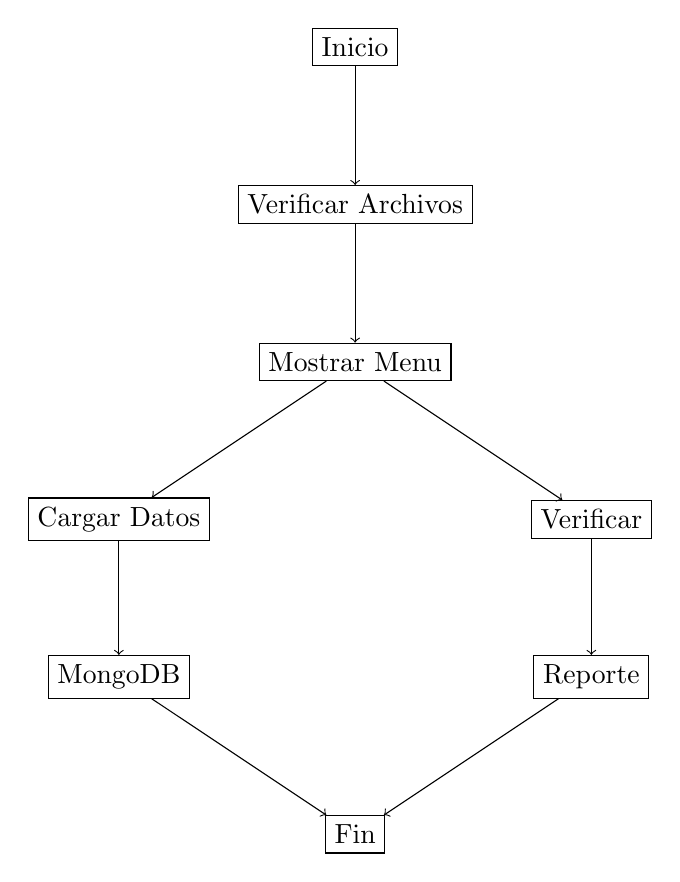
\begin{tikzpicture}[node distance=2cm]
    \node (start) [rectangle, draw] {Inicio};
    \node (check) [rectangle, draw, below of=start] {Verificar Archivos};
    \node (menu) [rectangle, draw, below of=check] {Mostrar Menu};
    \node (load) [rectangle, draw, below of=menu, xshift=-3cm] {Cargar Datos};
    \node (verify) [rectangle, draw, below of=menu, xshift=3cm] {Verificar};
    \node (mongo) [rectangle, draw, below of=load] {MongoDB};
    \node (report) [rectangle, draw, below of=verify] {Reporte};
    \node (end) [rectangle, draw, below of=mongo, xshift=3cm] {Fin};
    
    \draw [->] (start) -- (check);
    \draw [->] (check) -- (menu);
    \draw [->] (menu) -- (load);
    \draw [->] (menu) -- (verify);
    \draw [->] (load) -- (mongo);
    \draw [->] (verify) -- (report);
    \draw [->] (mongo) -- (end);
    \draw [->] (report) -- (end);
  \end{tikzpicture}
  \caption{Flujo del sistema de carga de datos}
\end{figure}

% ── IMPLEMENTACIÓN ──────────────────────────
\section{Implementacion}

\subsection{Verificacion y Descarga de Archivos}

El sistema verifica automáticamente la existencia de dos archivos críticos:

\begin{enumerate}
  \item \textbf{MunicipiosPDET.xlsx}: Contiene los códigos DANE de los municipios PDET
  \item \textbf{MGN\_2025\_COLOMBIA/.../shapefile.shp}: Contiene la información geográfica de Colombia
\end{enumerate}

Si alguno de estos archivos no existe, el sistema los descarga automáticamente desde las fuentes oficiales:

\begin{lstlisting}[caption=Descarga automática de archivos]
def download_file(url: str, filename: str) -> bool:
    """Descarga un archivo desde una URL."""
    try:
        print(f"Descargando {filename}...")
        response = requests.get(url, stream=True, timeout=30)
        response.raise_for_status()
        
        total_size = int(response.headers.get('content-length', 0))
        downloaded = 0
        
        with open(filename, 'wb') as f:
            for chunk in response.iter_content(chunk_size=8192):
                if chunk:
                    f.write(chunk)
                    downloaded += len(chunk)
        print(f"{filename} descargado exitosamente")
        return True
    except Exception as e:
        print(f"Error al descargar {filename}: {e}")
        return False
\end{lstlisting}

\subsection{Carga de Datos en MongoDB}

La función principal \texttt{run\_ingestion} realiza los siguientes pasos:

\begin{lstlisting}[caption=Proceso de ingesta de datos]
def run_ingestion(shapefile_path: str):
    client = MongoClient(MONGO_URI)
    col = client[DB_NAME][COL_NAME]

    # 1. Cargar codigos PDET desde Excel
    pdet_codes = load_pdet_codes(PDET_XLSX)

    # 2. Leer shapefile
    gdf = gpd.read_file(shapefile_path)
    
    # 3. Calcular area en m2
    gdf["area_m2"] = gdf.to_crs(epsg=9377).geometry.area

    # 4. Reproyectar a WGS84 para MongoDB 2dsphere
    if gdf.crs.to_epsg() != 4326:
        gdf = gdf.to_crs(epsg=4326)

    # 5. Filtrar municipios PDET
    gdf_pdet = gdf[gdf["dane_code"].isin(pdet_codes)].copy()
    
    # 6. Cargar en MongoDB
    for doc in records:
        col.update_one({"dane_code": doc["dane_code"]}, 
                      {"$set": doc}, upsert=True)
\end{lstlisting}

Cada documento almacenado contiene:
\begin{itemize}
  \item \textbf{dane\_code}: Código DIVIPOLA del municipio
  \item \textbf{name}: Nombre del municipio
  \item \textbf{department}: Nombre del departamento
  \item \textbf{is\_pdet}: Indicador booleano (siempre True)
  \item \textbf{geometry}: Geometría en formato GeoJSON
  \item \textbf{area\_m2}: Área del municipio en metros cuadrados
  \item \textbf{source}: Fuente de los datos (MGN2025)
  \item \textbf{ingested\_at}: Timestamp de carga
\end{itemize}

\subsection{Creacion de Índices}

Se crea automáticamente un índice geoespacial 2dsphere:

\begin{lstlisting}[caption=Creacion de indice 2dsphere]
col.create_index([("geometry", GEOSPHERE)])
\end{lstlisting}

Este índice permite realizar consultas geoespaciales eficientes.

% ── RESULTADOS ──────────────────────────────
\section{Resultados}

\subsection{Ejecucion del Sistema}

\begin{figure}[H]
  \centering
  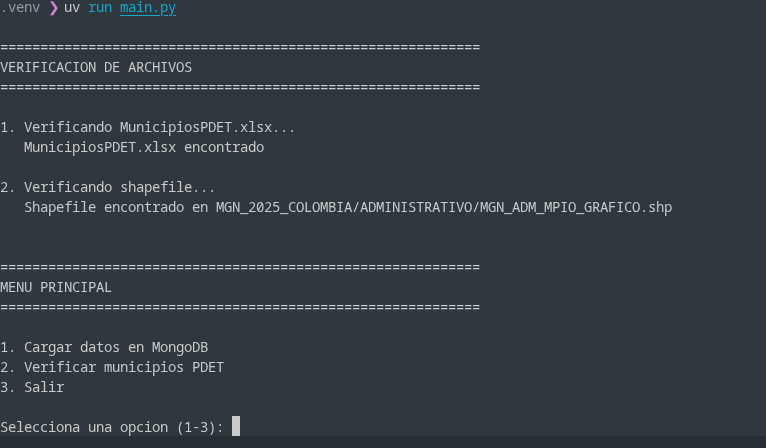
\includegraphics[width=0.9\linewidth]{placeholder_menu.png}
  \caption{Menu principal del sistema}
  \label{fig:menu}
\end{figure}

\begin{figure}[H]
  \centering
  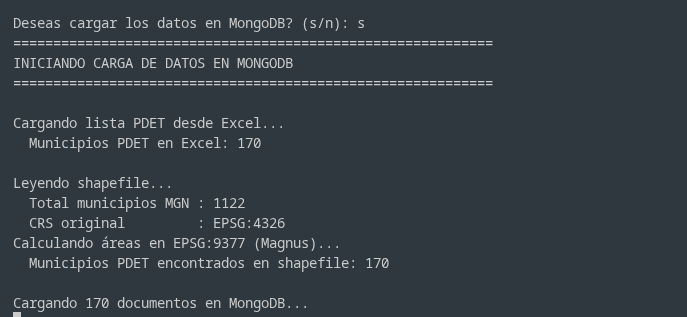
\includegraphics[width=0.9\linewidth]{placeholder_loading.png}
  \caption{Proceso de carga de datos en MongoDB}
  \label{fig:loading}
\end{figure}

\subsection{Verificacion de Integridad}

La función \texttt{verify\_pdet\_municipalities()} verifica que todos los municipios PDET fueron cargados correctamente:

\begin{lstlisting}[caption=Verificacion de municipios PDET]
def verify_pdet_municipalities():
    # Cargar codigos esperados desde Excel
    pdet_codes_excel = load_pdet_codes(PDET_XLSX)
    
    # Obtener codigos en MongoDB
    pdet_mongo = set(doc["dane_code"] for doc in 
                     col.find({"is_pdet": True}))
    
    # Detectar discrepancias
    missing = pdet_codes_excel - pdet_mongo
    extra = pdet_mongo - pdet_codes_excel
    
    # Reportar resultado
    if not missing and not extra:
        print("Verificacion exitosa")
        return True
    else:
        print("Se encontraron discrepancias")
        return False
\end{lstlisting}

\begin{figure}[H]
  \centering
  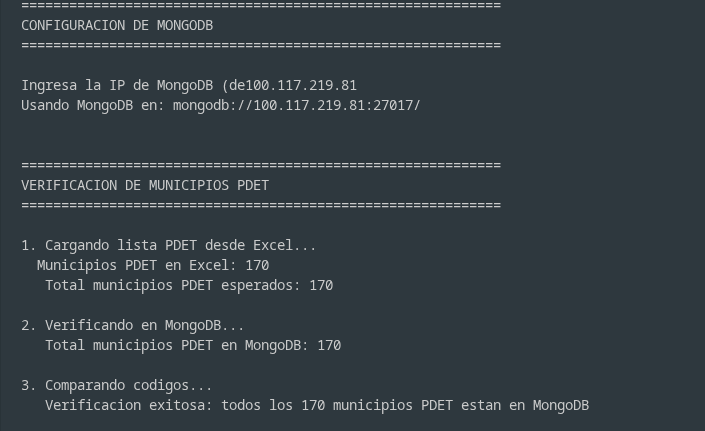
\includegraphics[width=0.9\linewidth]{foto_verificacion_datos.png}
  \caption{Resultado de la verificacion de integridad}
  \label{fig:verification}
\end{figure}

% ── USO DEL SISTEMA ─────────────────────────
\section{Uso del Sistema}

\subsection{Instalacion de Dependencias}

\begin{lstlisting}[caption=Instalacion de paquetes requeridos]
pip install pandas geopandas pymongo requests
\end{lstlisting}

\subsection{Ejecucion Principal}

\begin{lstlisting}[caption=Ejecucion del programa]
python main.py
\end{lstlisting}

El sistema presentará un menú interactivo con las opciones:
\begin{enumerate}
  \item Cargar datos en MongoDB
  \item Verificar municipios PDET
  \item Salir
\end{enumerate}

\subsection{Flujo de Interaccion}

\begin{lstlisting}[caption=Ejemplo de flujo interactivo]
============================================================
MENU PRINCIPAL
============================================================

1. Cargar datos en MongoDB
2. Verificar municipios PDET
3. Salir

Selecciona una opcion (1-3): 1
============================================================
CONFIGURACION DE MONGODB
============================================================

Ingresa la IP de MongoDB (deja en blanco para localhost):

Usando MongoDB local: mongodb://localhost:27017/

============================================================
OPCIONES DE CARGA DE DATOS
============================================================

Deseas cargar los datos en MongoDB? (s/n): s
\end{lstlisting}

% ── CONCLUSIONES ────────────────────────────
\section{Conclusiones}

Durante esta semana se logró implementar con éxito un sistema robusto de carga de datos geográficos en MongoDB. Los puntos destacados incluyen:

\begin{itemize}
  \item Automatización completa de descarga y verificación de archivos
  \item Pipeline de ingesta modular y escalable
  \item Implementación de índices geoespaciales para consultas eficientes
  \item Sistema de verificación de integridad de datos
  \item Interfaz interactiva amigable con el usuario
\end{itemize}

El sistema está listo para producción y permite la carga correcta de todos los municipios PDET en MongoDB con garantía de integridad de datos.

\end{document}
